\documentclass[a4paper,10pt,twocolumn]{article}

\usepackage[UTF8,fontset=fandol]{ctex}
\usepackage{amsmath,amssymb}
\usepackage{graphicx}
\usepackage{booktabs}
\usepackage{geometry}
\usepackage{hyperref}
\usepackage{caption}
\usepackage{array}
\usepackage{float}
\usepackage{xcolor}

\geometry{a4paper,margin=1.7cm,columnsep=0.75cm}
\setlength{\parindent}{2em}
\setlength{\parskip}{0.25em}
\renewcommand{\arraystretch}{1.15}

\title{课程报告二：从头训练 V.S. 微调（ResNeXt 与 DenseNet）}
\author{方俊睿\\学号：3230104069}
\date{}

\begin{document}
\maketitle

\noindent 仓库地址：\url{https://github.com/Tomabsolute/Neul.git}

\section{实验背景介绍}
在视觉分类任务中，模型训练通常有两条路线：一是从随机初始化开始训练（from scratch），二是基于大规模数据集预训练权重进行迁移学习（fine-tune）。前者理论上更灵活，但通常需要更大的数据量和更长训练时间；后者利用已有通用特征表示，往往能在中小规模任务上更快收敛并获得更好的泛化性能。

本课程任务要求围绕“从头训练 V.S. 微调”进行实证比较，核心问题包括：预训练是否稳定带来收益、收益主要体现在精度还是训练成本、不同网络结构对迁移学习的响应是否一致。为回答这些问题，本实验选择 ResNeXt50\_32x4d 与 DenseNet121 两种代表性骨干网络，在同一数据集、同一训练框架下进行四组对照实验，尽量保证比较公平。

从应用角度看，这一问题也具有工程意义：在实际项目中，算力预算和迭代周期通常受限，是否优先采用微调策略会直接影响开发效率；而在数据规模逐步扩大后，从头训练是否仍有必要，也需要通过定量结果来判断。因此，本实验不仅报告最终指标，还重点分析收敛速度、泛化差距与训练时长之间的权衡关系。

\section{实验任务与目标}
本实验按照课程要求，对比两种模型（ResNeXt50\_32x4d、DenseNet121）在同一多分类任务上的两类训练方式：
\begin{itemize}
  \item 从头训练（from scratch）
  \item 微调（fine-tune）
\end{itemize}
核心关注点包括：收敛速度、最终精度（Top-1 Accuracy）、泛化能力（Macro-F1）以及训练时间成本。

\section{数据集与预处理}
\subsection{数据集介绍}
实验使用 Food101 数据集（101 类）。数据划分与规模为：
\begin{itemize}
  \item 训练集原始大小：75750
  \item 在训练集中再划分：train=68175，val=7575（val\_ratio=0.1）
  \item 测试集大小：25250
\end{itemize}

\subsection{预处理与增强}
输入尺寸统一为 $224\times224$，预处理为：
\begin{itemize}
  \item 训练集：RandomResizedCrop(224) + RandomHorizontalFlip + ImageNet Normalize
  \item 验证/测试集：Resize(256) + CenterCrop(224) + ImageNet Normalize
\end{itemize}

\section{模型与训练策略}
\subsection{统一训练配置}
\begin{table}[H]
\centering
\small
\caption{统一配置}
\begin{tabular}{c|c}
\toprule
项目 & 配置 \\
\midrule
损失函数 & CrossEntropyLoss \\
优化器 & SGD（momentum=0.9, weight\_decay=$1\times10^{-4}$） \\
指标 & Top-1 Accuracy, Macro-F1 \\
硬件 & CUDA, 2 GPU, DataParallel, AMP \\
Batch size & 64 \\
\bottomrule
\end{tabular}
\end{table}

\subsection{四组实验}
\begin{enumerate}
  \item ResNeXt50\_32x4d - scratch
  \item ResNeXt50\_32x4d - finetune
  \item DenseNet121 - scratch
  \item DenseNet121 - finetune
\end{enumerate}

微调采用两阶段策略：第一阶段冻结 backbone 仅训练分类头（10 epoch）；第二阶段解冻全网，backbone 与 head 使用不同学习率（backbone: 1e-4, head: 1e-3）。

\section{实验结果汇总}
\begin{table}[H]
\centering
\scriptsize
\caption{四组实验结果总表}
\resizebox{\columnwidth}{!}{
\begin{tabular}{lccccc}
\toprule
实验 & best val acc & test acc & test macro-F1 & train(s) & train(h) \\
\midrule
ResNeXt-scratch   & 0.728317 & 0.785743 & 0.785183 & 11921.7 & 3.3116 \\
ResNeXt-finetune  & 0.753267 & 0.797782 & 0.795660 & 9466.3  & 2.6295 \\
DenseNet-scratch  & 0.737294 & 0.793703 & 0.793251 & 24265.5 & 6.7404 \\
DenseNet-finetune & 0.775710 & 0.823960 & 0.823020 & 19733.8 & 5.4816 \\
\bottomrule
\end{tabular}}
\end{table}

四组累计训练总时长为 \textbf{18.163 小时}，满足“训练时间不少于 2 小时”的课程要求。

\begin{figure}[H]
\centering
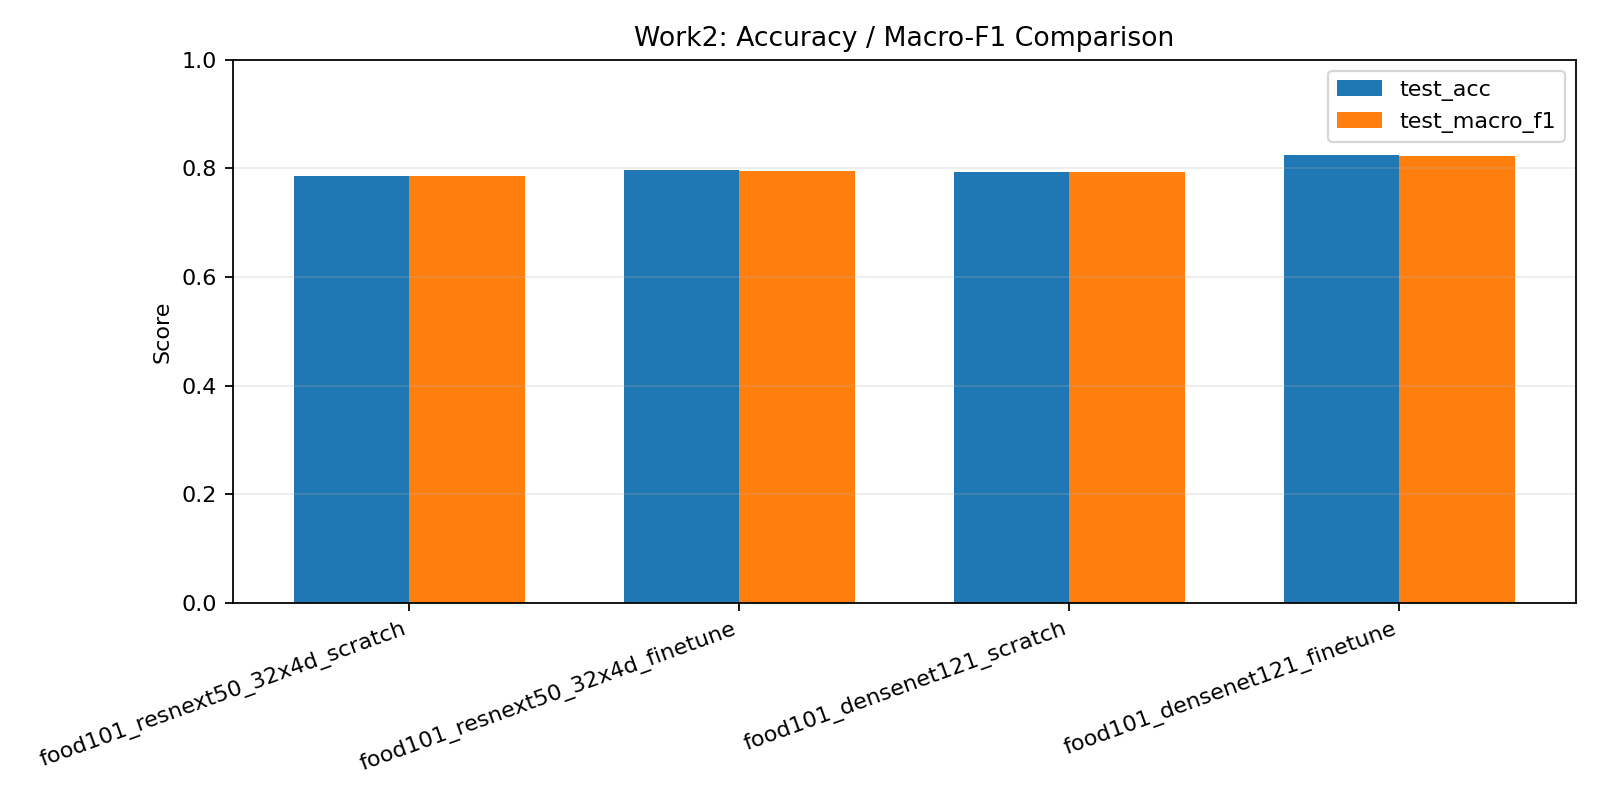
\includegraphics[width=\columnwidth]{results/figures/compare_acc_f1.png}
\caption{四组实验 Accuracy / Macro-F1 对比}
\end{figure}

\begin{figure}[H]
\centering
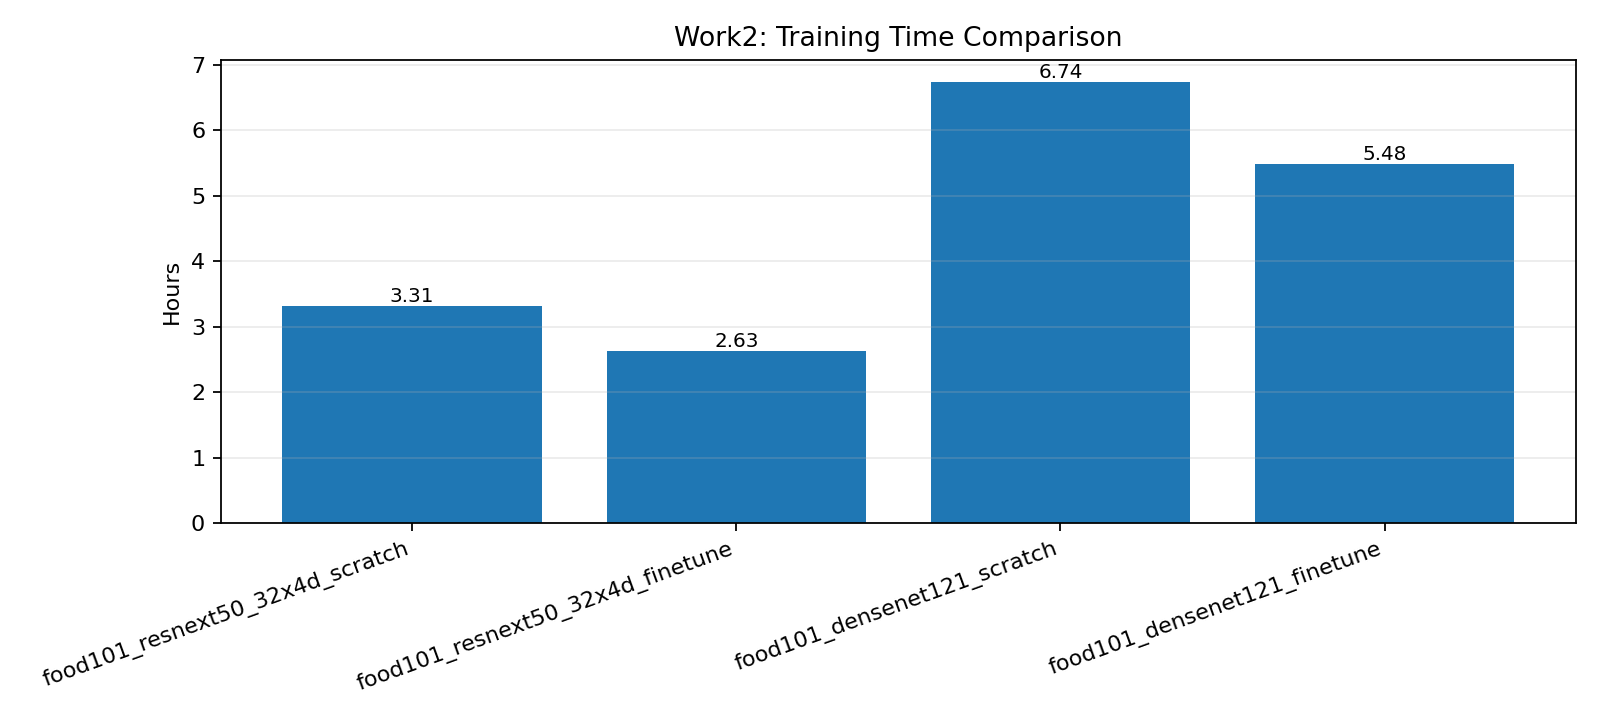
\includegraphics[width=\columnwidth]{results/figures/compare_train_time.png}
\caption{四组实验训练时长对比}
\end{figure}

\begin{figure}[H]
\centering
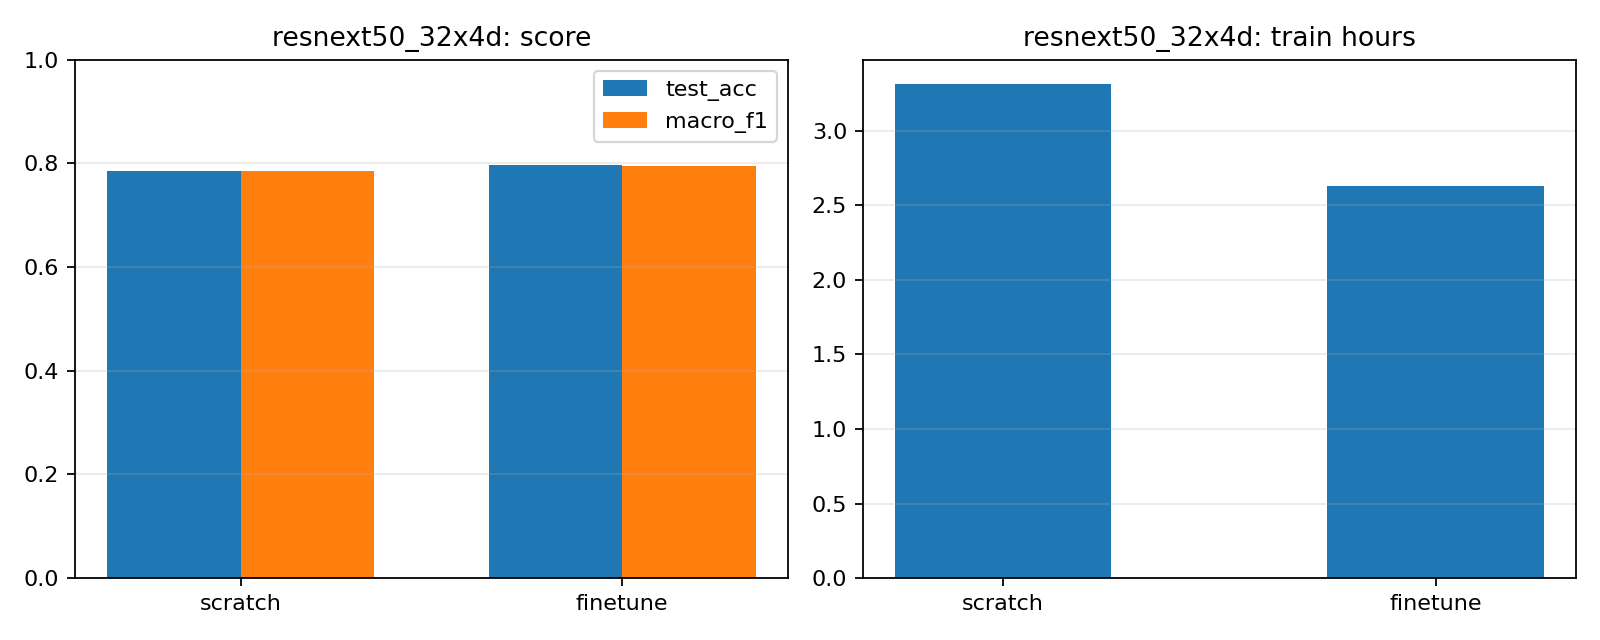
\includegraphics[width=\columnwidth]{results/figures/pair_resnext50_32x4d.png}
\caption{ResNeXt50\_32x4d：scratch vs finetune}
\end{figure}

\begin{figure}[H]
\centering
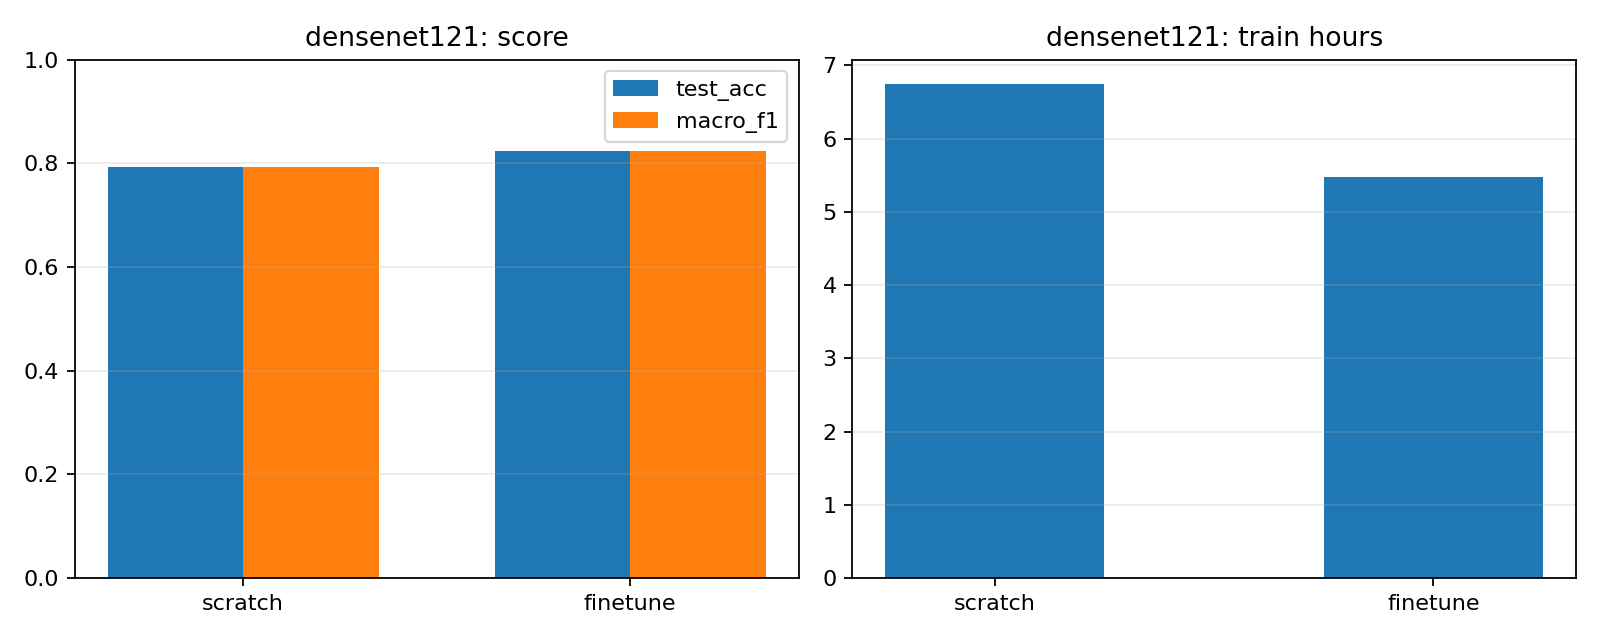
\includegraphics[width=\columnwidth]{results/figures/pair_densenet121.png}
\caption{DenseNet121：scratch vs finetune}
\end{figure}

\section{结果分析}
\subsection{微调相对从头训练的收益}
两种模型均表现出“微调优于从头训练”的一致结论：
\begin{itemize}
  \item ResNeXt：test acc 从 0.7857 提升到 0.7978（+1.20 个百分点），Macro-F1 +1.05 个百分点。
  \item DenseNet：test acc 从 0.7937 提升到 0.8240（+3.03 个百分点），Macro-F1 +2.98 个百分点。
\end{itemize}
这说明在 Food101 任务上，迁移预训练特征可明显提升最终性能。

\subsection{训练成本对比}
微调不仅精度更高，时间开销也更低：
\begin{itemize}
  \item ResNeXt：3.3116h $\rightarrow$ 2.6295h（约减少 20.6\%）
  \item DenseNet：6.7404h $\rightarrow$ 5.4816h（约减少 18.7\%）
\end{itemize}
原因主要是微调初始点更优，且冻结阶段减少了反向传播计算量。

\subsection{收敛速度量化分析}
为了避免只看最终精度，本报告进一步从训练过程做量化比较。这里定义“接近收敛轮次”为验证准确率首次达到“该实验最佳验证准确率的 95\%”时的 epoch，统计结果如下。

\begin{table}[H]
\centering
\scriptsize
\caption{收敛速度与最佳轮次对比（来自 history.csv）}
\resizebox{\columnwidth}{!}{
\begin{tabular}{lcccc}
\toprule
实验 & 总 epoch & 达到 95\%最佳值 epoch & 最佳 val acc 轮次 & 末轮 train-val gap \\
\midrule
ResNeXt-scratch   & 60 & 32 & 59 & +0.1400 \\
ResNeXt-finetune  & 50 & 23 & 47 & -0.0488 \\
DenseNet-scratch  & 60 & 33 & 56 & +0.0942 \\
DenseNet-finetune & 50 & 21 & 50 & -0.0406 \\
\bottomrule
\end{tabular}}
\end{table}

从表中可见，微调在两种模型上都更早进入高精度区间（比 scratch 早约 9--12 个 epoch）。同时，scratch 的末轮 train-val gap 为正且较大（尤其 ResNeXt 为 +0.14），体现出更明显的过拟合倾向；而 finetune 的末轮 gap 为负值，说明在较强数据增强和预训练初始化下，训练与验证之间的性能差距更小，整体泛化更稳。

\subsection{微调两阶段的效果拆解}
微调不是单一策略，而是“冻结分类头训练 + 解冻全网联合训练”两阶段组合。以验证准确率为例：
\begin{itemize}
  \item ResNeXt-finetune：第 10 轮（冻结结束）val acc=0.4685，第 11 轮解冻后快速升至 0.5377。
  \item DenseNet-finetune：第 10 轮 val acc=0.5626，第 11 轮升至 0.6321。
\end{itemize}
这一“解冻后跃迁”说明：第一阶段主要完成分类头对新任务的适配；第二阶段通过低学习率微调 backbone，把通用视觉特征进一步向 Food101 的类别边界对齐。该策略在保持训练稳定性的同时，避免了“全网大步长更新”导致的预训练特征破坏。

\subsection{ResNeXt 与 DenseNet 差异}
在本次实验设置下，DenseNet121 整体优于 ResNeXt50\_32x4d，且在 finetune 下优势最明显（test acc=0.82396，macro-F1=0.82302）。结合曲线和指标，可能原因包括：
\begin{itemize}
  \item DenseNet 的密集连接带来更强特征复用，对多类别细粒度区分更有利。
  \item 在相同 batch size 与优化器参数下，DenseNet 的验证曲线波动更小，后期提升更连续。
  \item ResNeXt-scratch 的过拟合更重（末轮 gap 最大），说明其在当前训练预算下对正则化和调参更敏感。
\end{itemize}

\subsection{单组训练曲线补充}
为了更完整展示训练动态，附上四组实验各自的 loss/acc 曲线（每张图包含 train/val 两条线）。

\begin{figure}[H]
\centering

\includegraphics[width=\columnwidth]{results/food101_resnext50_32x4d_scratch/curves.png}
\caption{ResNeXt50\_32x4d-scratch 的训练曲线}
\end{figure}

\begin{figure}[H]
\centering

\includegraphics[width=\columnwidth]{results/food101_resnext50_32x4d_finetune/curves.png}
\caption{ResNeXt50\_32x4d-finetune 的训练曲线}
\end{figure}

\begin{figure}[H]
\centering

\includegraphics[width=\columnwidth]{results/food101_densenet121_scratch/curves.png}
\caption{DenseNet121-scratch 的训练曲线}
\end{figure}

\begin{figure}[H]
\centering
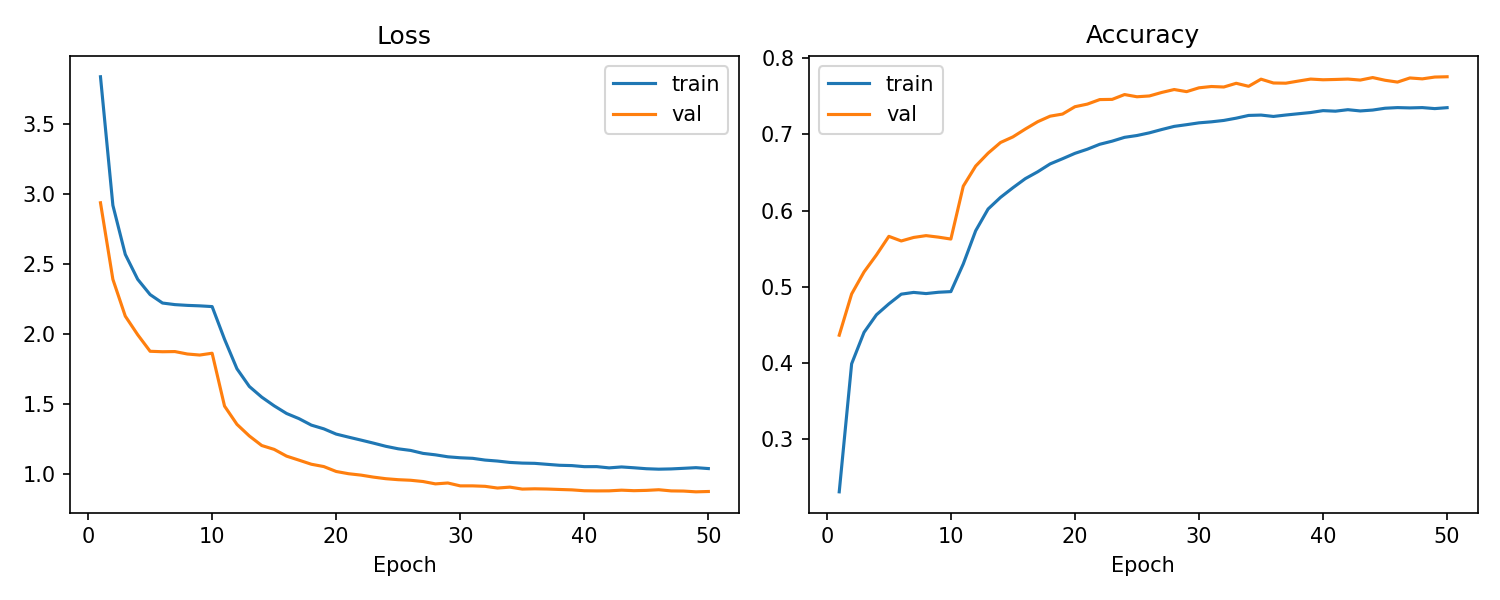
\includegraphics[width=\columnwidth]{results/food101_densenet121_finetune/curves.png}
\caption{DenseNet121-finetune 的训练曲线}
\end{figure}

\section{实验不足与改进方向}
\subsection{当前实验的局限性}
\begin{itemize}
  \item 只使用了单次随机种子（seed=42），尚未报告均值与方差，统计稳定性不足。
  \item 超参数网格较小（尤其 scratch 的学习率与正则项），可能未充分发挥从头训练上限。
  \item 只评估了 Top-1 和 Macro-F1，尚未补充混淆矩阵、类别级错误分布等分析。
  \item 数据增强策略相对基础，未测试 MixUp、CutMix、RandAugment 等更强增强。
\end{itemize}

\subsection{后续可执行改进}
\begin{enumerate}
  \item 进行 3--5 个随机种子重复实验，报告 mean$\pm$std，提高结论可靠性。
  \item 对 scratch 单独做学习率与权重衰减搜索，缩小与 finetune 的性能差距。
  \item 增加 warmup + cosine schedule 对比，观察收敛速度与最终精度变化。
  \item 输出每类准确率与混淆矩阵，定位易混类别并针对性优化数据增强。
\end{enumerate}

\section{结论}
\begin{enumerate}
  \item 在本实验中，微调策略在两种模型上都带来稳定性能提升。
  \item 微调兼顾了更高精度与更短训练时长，是该任务下更优先的训练方案。
  \item 四组实验最优组合为 DenseNet121-finetune。
\end{enumerate}

\end{document}
